\subsection{Energieversorgung}
Die einzelnen Komponenten benötigen für den Betrieb verschieden Spannungen. 
Diese werden mit der Energieversorgung bereitgestellt. Dazu werden Netzteile 
aus Servern verwendet. Davon werden vier in Serie geschaltet um die notwendige 
Spannung von 48\si{\volt} zu erreichen. Um Kurzschlüsse zu vermeiden, müssen 
die Netzteile potentialfrei gemacht werden. Bei den verwendeten Netzteilen vom 
Typ PS-3701-1 von HP wird die Sekundärseite mit einer Schraube elektrisch mit 
dem Gehäuse verbunden. Das Gehäuse ist mit PE verbunden und somit geerdet. 
Diese Schraube wird durch eine Kunststoffschraube ersetzt. Ausserdem ist der 
Abstand vom Gehäuse zur Platine an der Austrittsstelle der Platine sehr klein 
und kann zu unerwünschten Kurzschlüssen führen. Daher wird mit einem 
isolierenden Streifen aus FR4 einem allfälligen Kurzschluss vorgebeugt. 
\begin{figure}[h!]
    \begin{minipage}{0.5\textwidth}
        \centering
        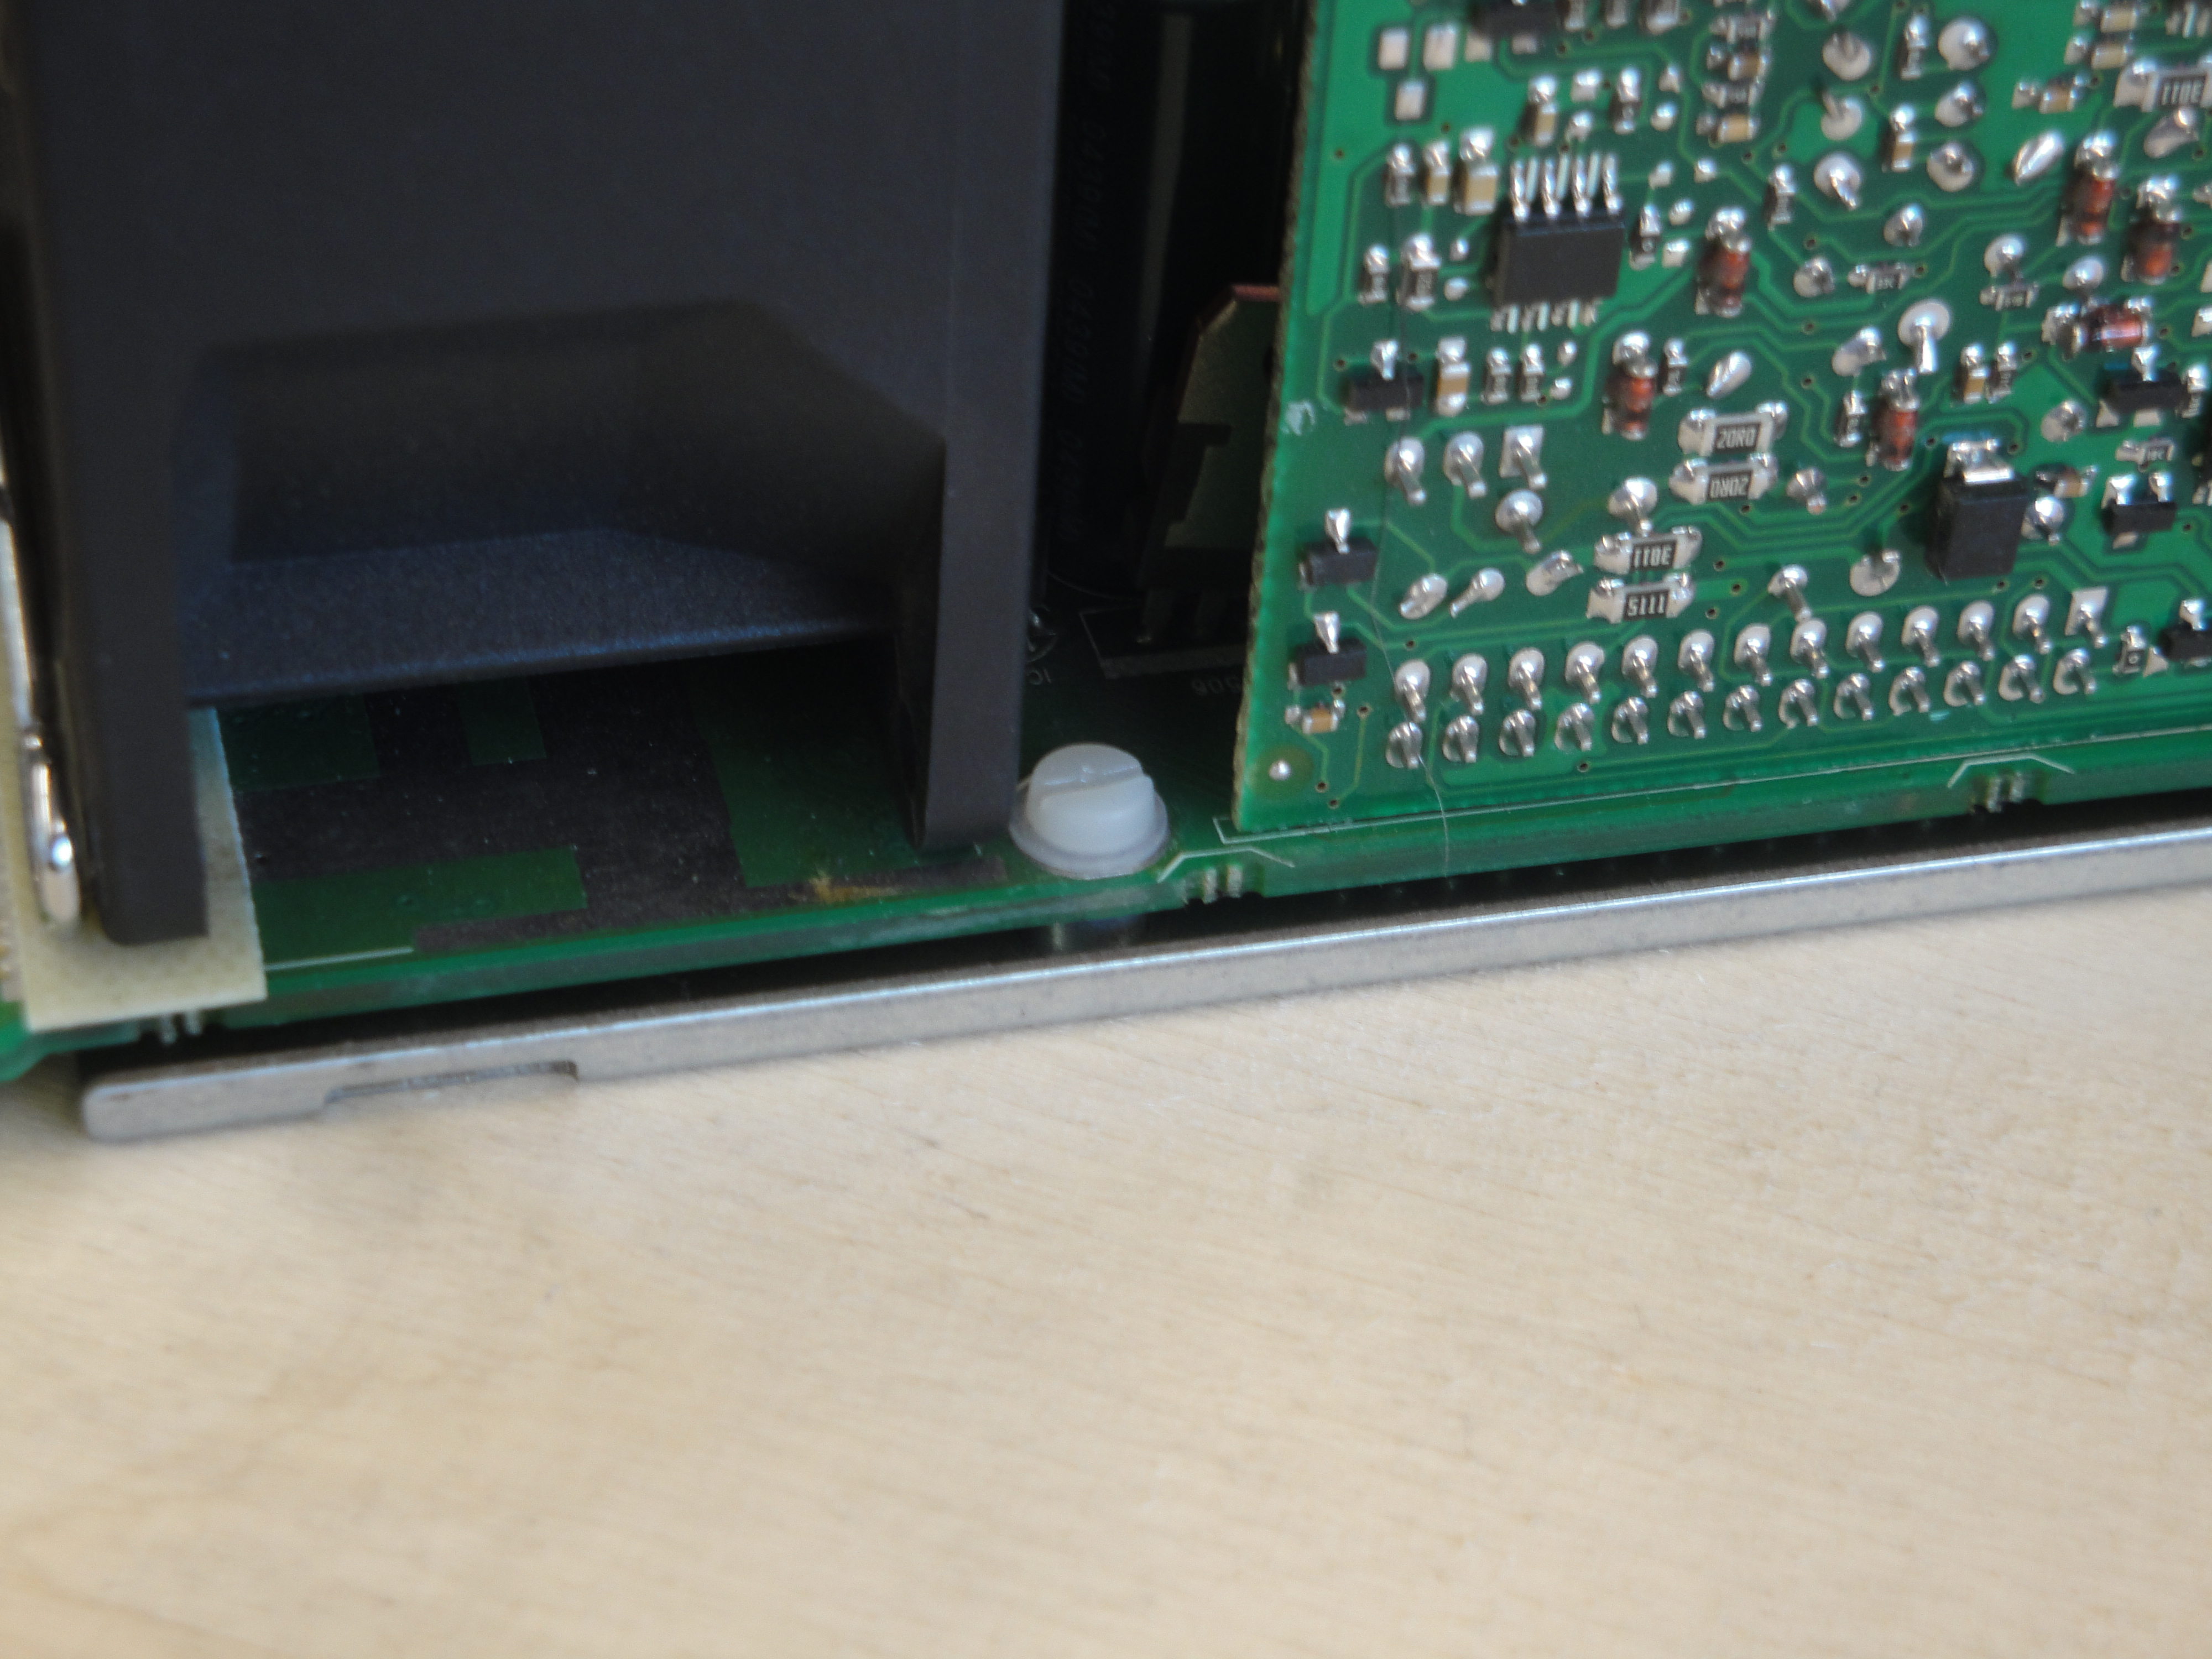
\includegraphics[width=0.8\textwidth]{fig/DSC02937.JPG}
        \caption*{Kunststoffschraube}
        \label{fig:e_sup_mod_screw}
    \end{minipage}
    \begin{minipage}{0.5\textwidth}
        \centering
        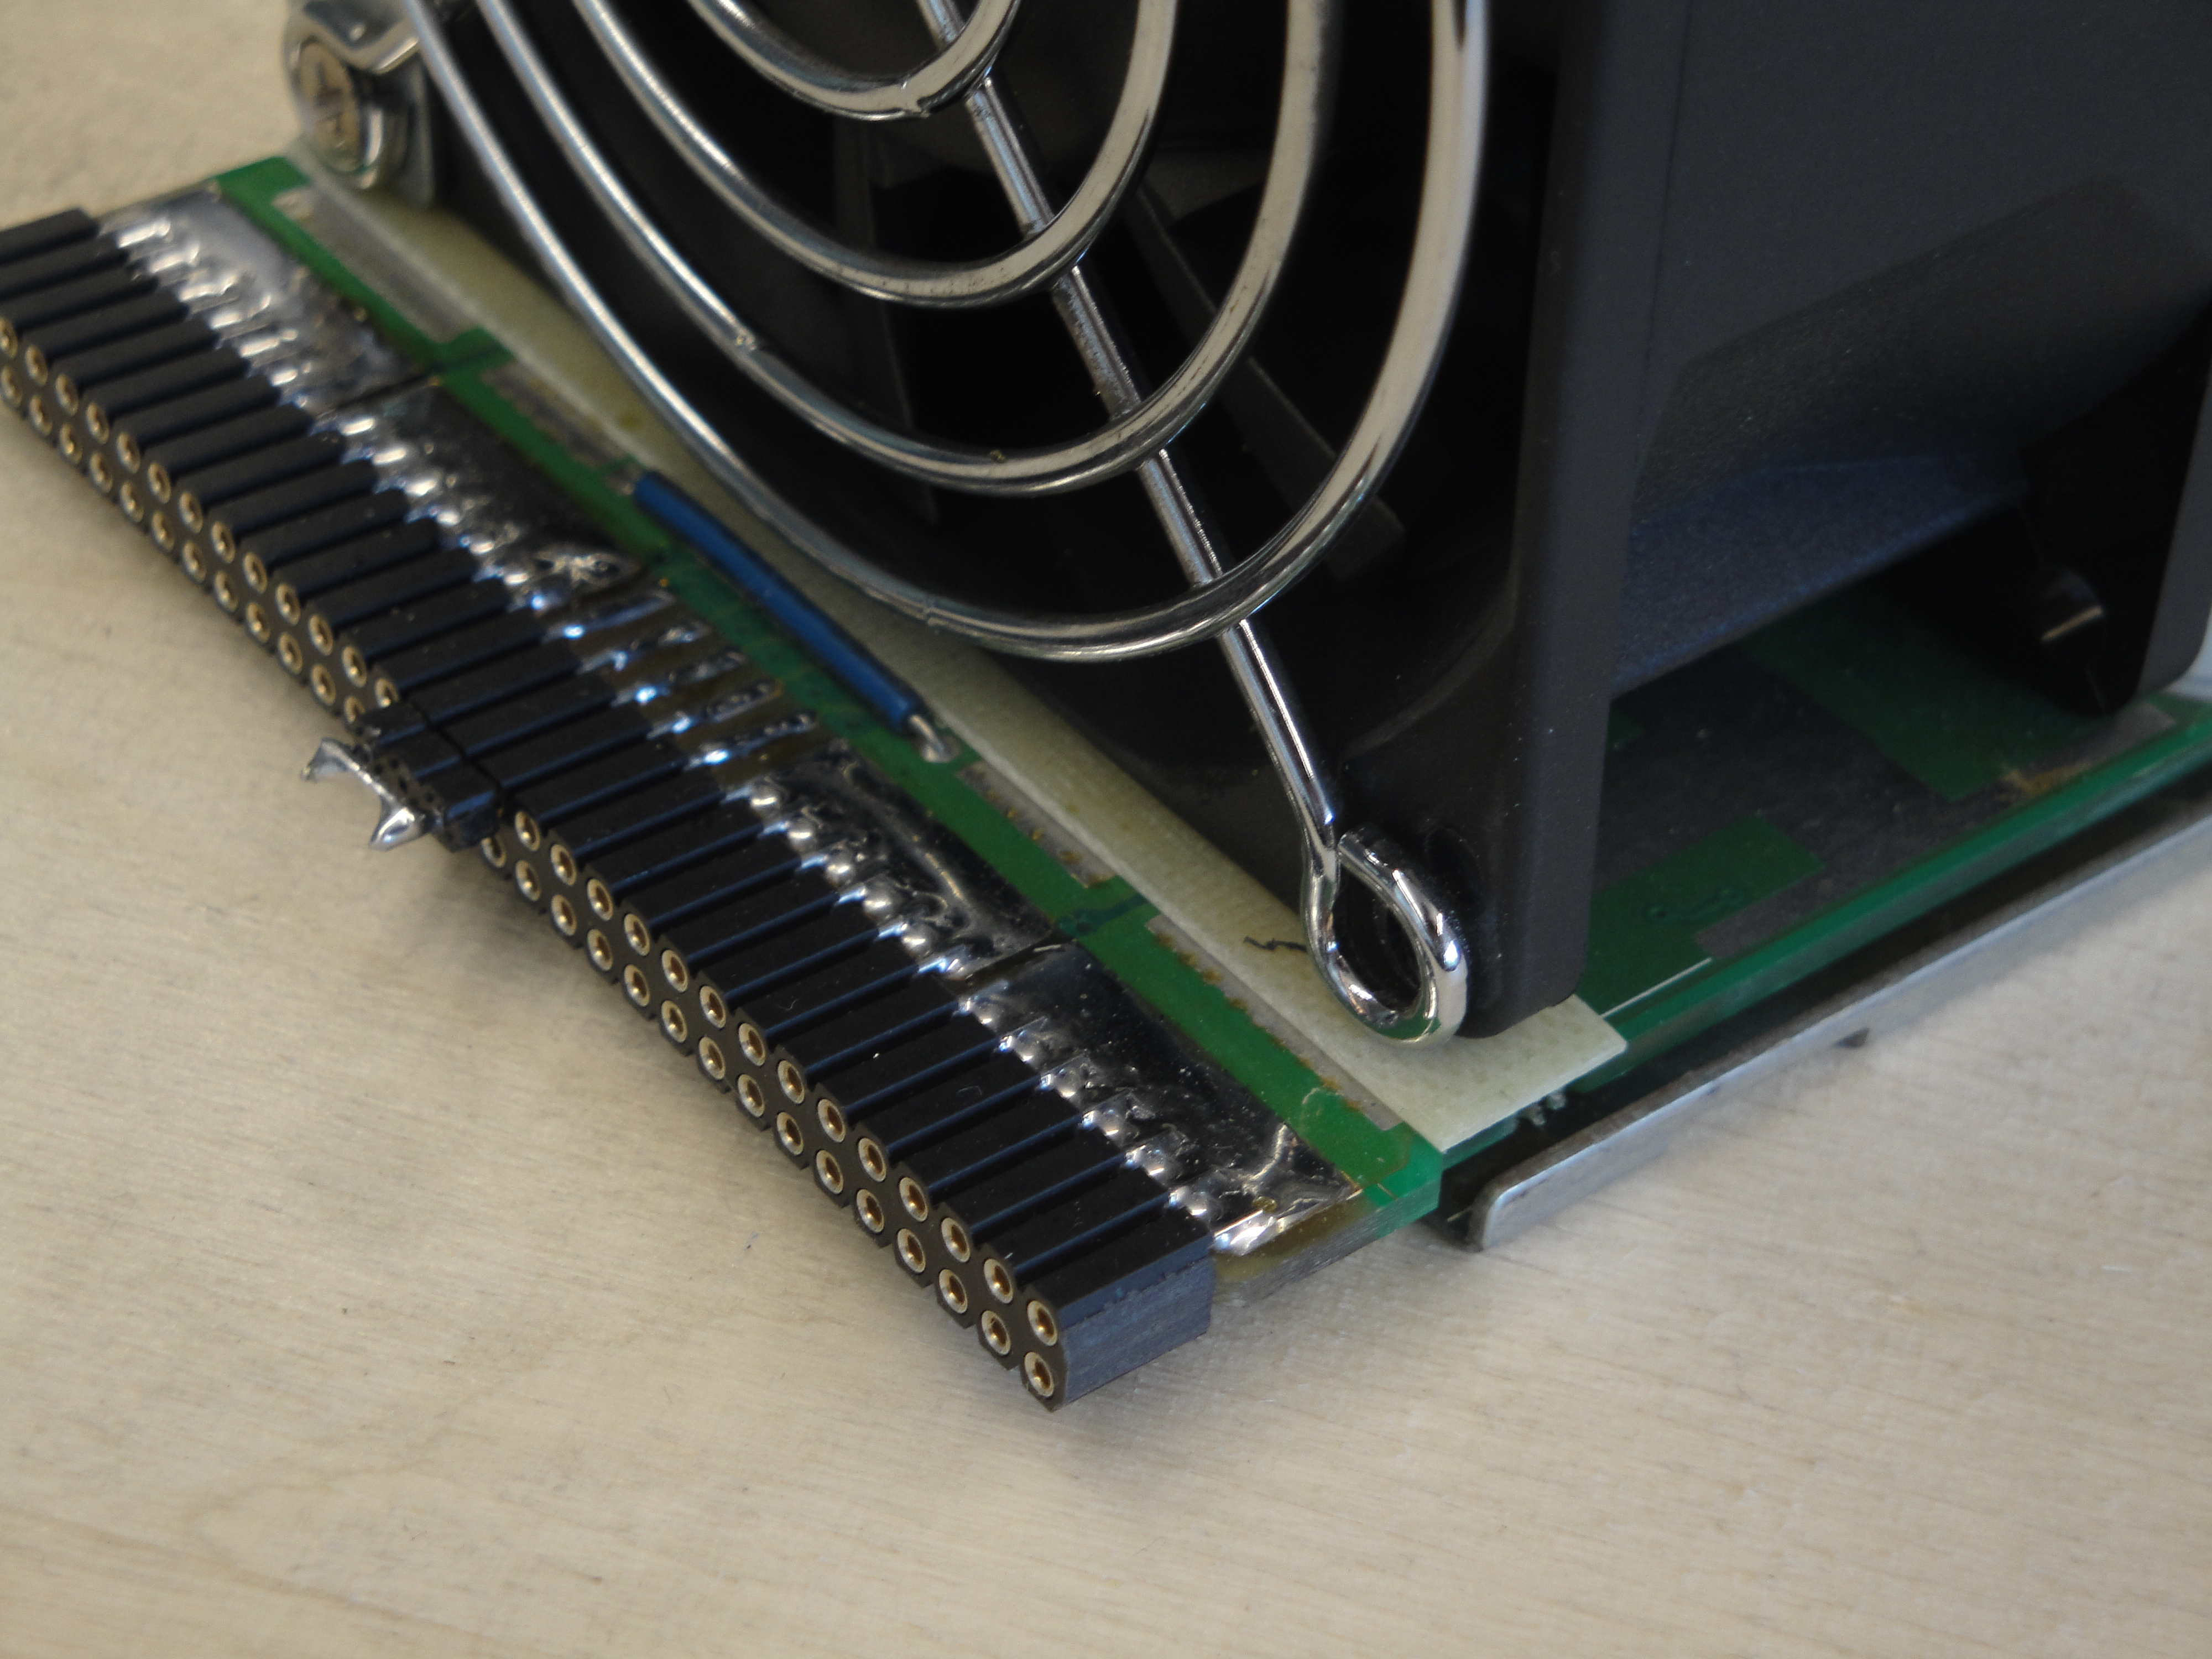
\includegraphics[width=0.8\textwidth]{fig/DSC02938.JPG}
        \caption*{Isolierender Streifen aus FR4}
        \label{fig:e_sup_mod_strip}
    \end{minipage}
    \caption{Modifikationen zur galvanischen Trennung der Sekundärseite der Netzteile}
    \label{fig:e_sup_mod}
\end{figure}

\noindent Die Netzteile werden auf einer Grundplatte aus Holz befestigt. Dazu 
werden entsprechende Ausschnitte gefräst. An die sekundärseitigen Anschlüsse 
werden Buchsenleisten angelötet, um die Verkabelung flexibler gestalten zu 
können. Die Netzteile werden mittels Stiftleisten in Serie geschaltet und die 
Spannungen 12\si{\volt}, 24\si{\volt} und 48\si{\volt} auf eine Steckmatrix 
verbunden. Mittels dieser Steckmatrix ist es möglich, für jeden Motor die 
Versorgungsspannung einzeln festzulegen. Die Konfiguration der einzelnen 
Komponenten ist ein \autoref{tab:e_sup_volt} ersichtlich. Jede Leitung wird 
einzeln mit einer Schmelzsicherung abgesichert. Die Versorgungsleitung und die 
zugehörige Masseleitung jeder Komponente werden jeweils mit dem gleichen Strom 
abgesichert. Um sicherzustellen, dass die Sicherung der Versorgungsleitung vor 
der Sicherung der Masseleitung auslöst, wird die Versorgungsleitung flink, die 
Masseleitung hingegen träge abgesichert. 
\begin{table}[h!]
    \centering
    \begin{zebratabular}{lll}
    \rowcolor{gray}
    Komponente                  & Versorgungsspannung   & Strom (Sicherung) \\
    Schrittmotoransteuerung     & 24\si{\volt}          & 500\si{\milli\ampere} \\
    BLDC Motor Ansteuerung      & 24\si{\volt}          & 10\si{\ampere} \\
    Gleichstrommotoransteuerung & 12\si{\volt}          & 1\si{\ampere} \\
    Controllerboard             &  5\si{\volt} (fix)    & 100\si{\milli\ampere} \\
    \end{zebratabular}
    \caption{Versorgungsspannung der einzelnen Komponenten}
    \label{tab:e_sup_volt}
\end{table}
\begin{figure}[h!]
    \centering
    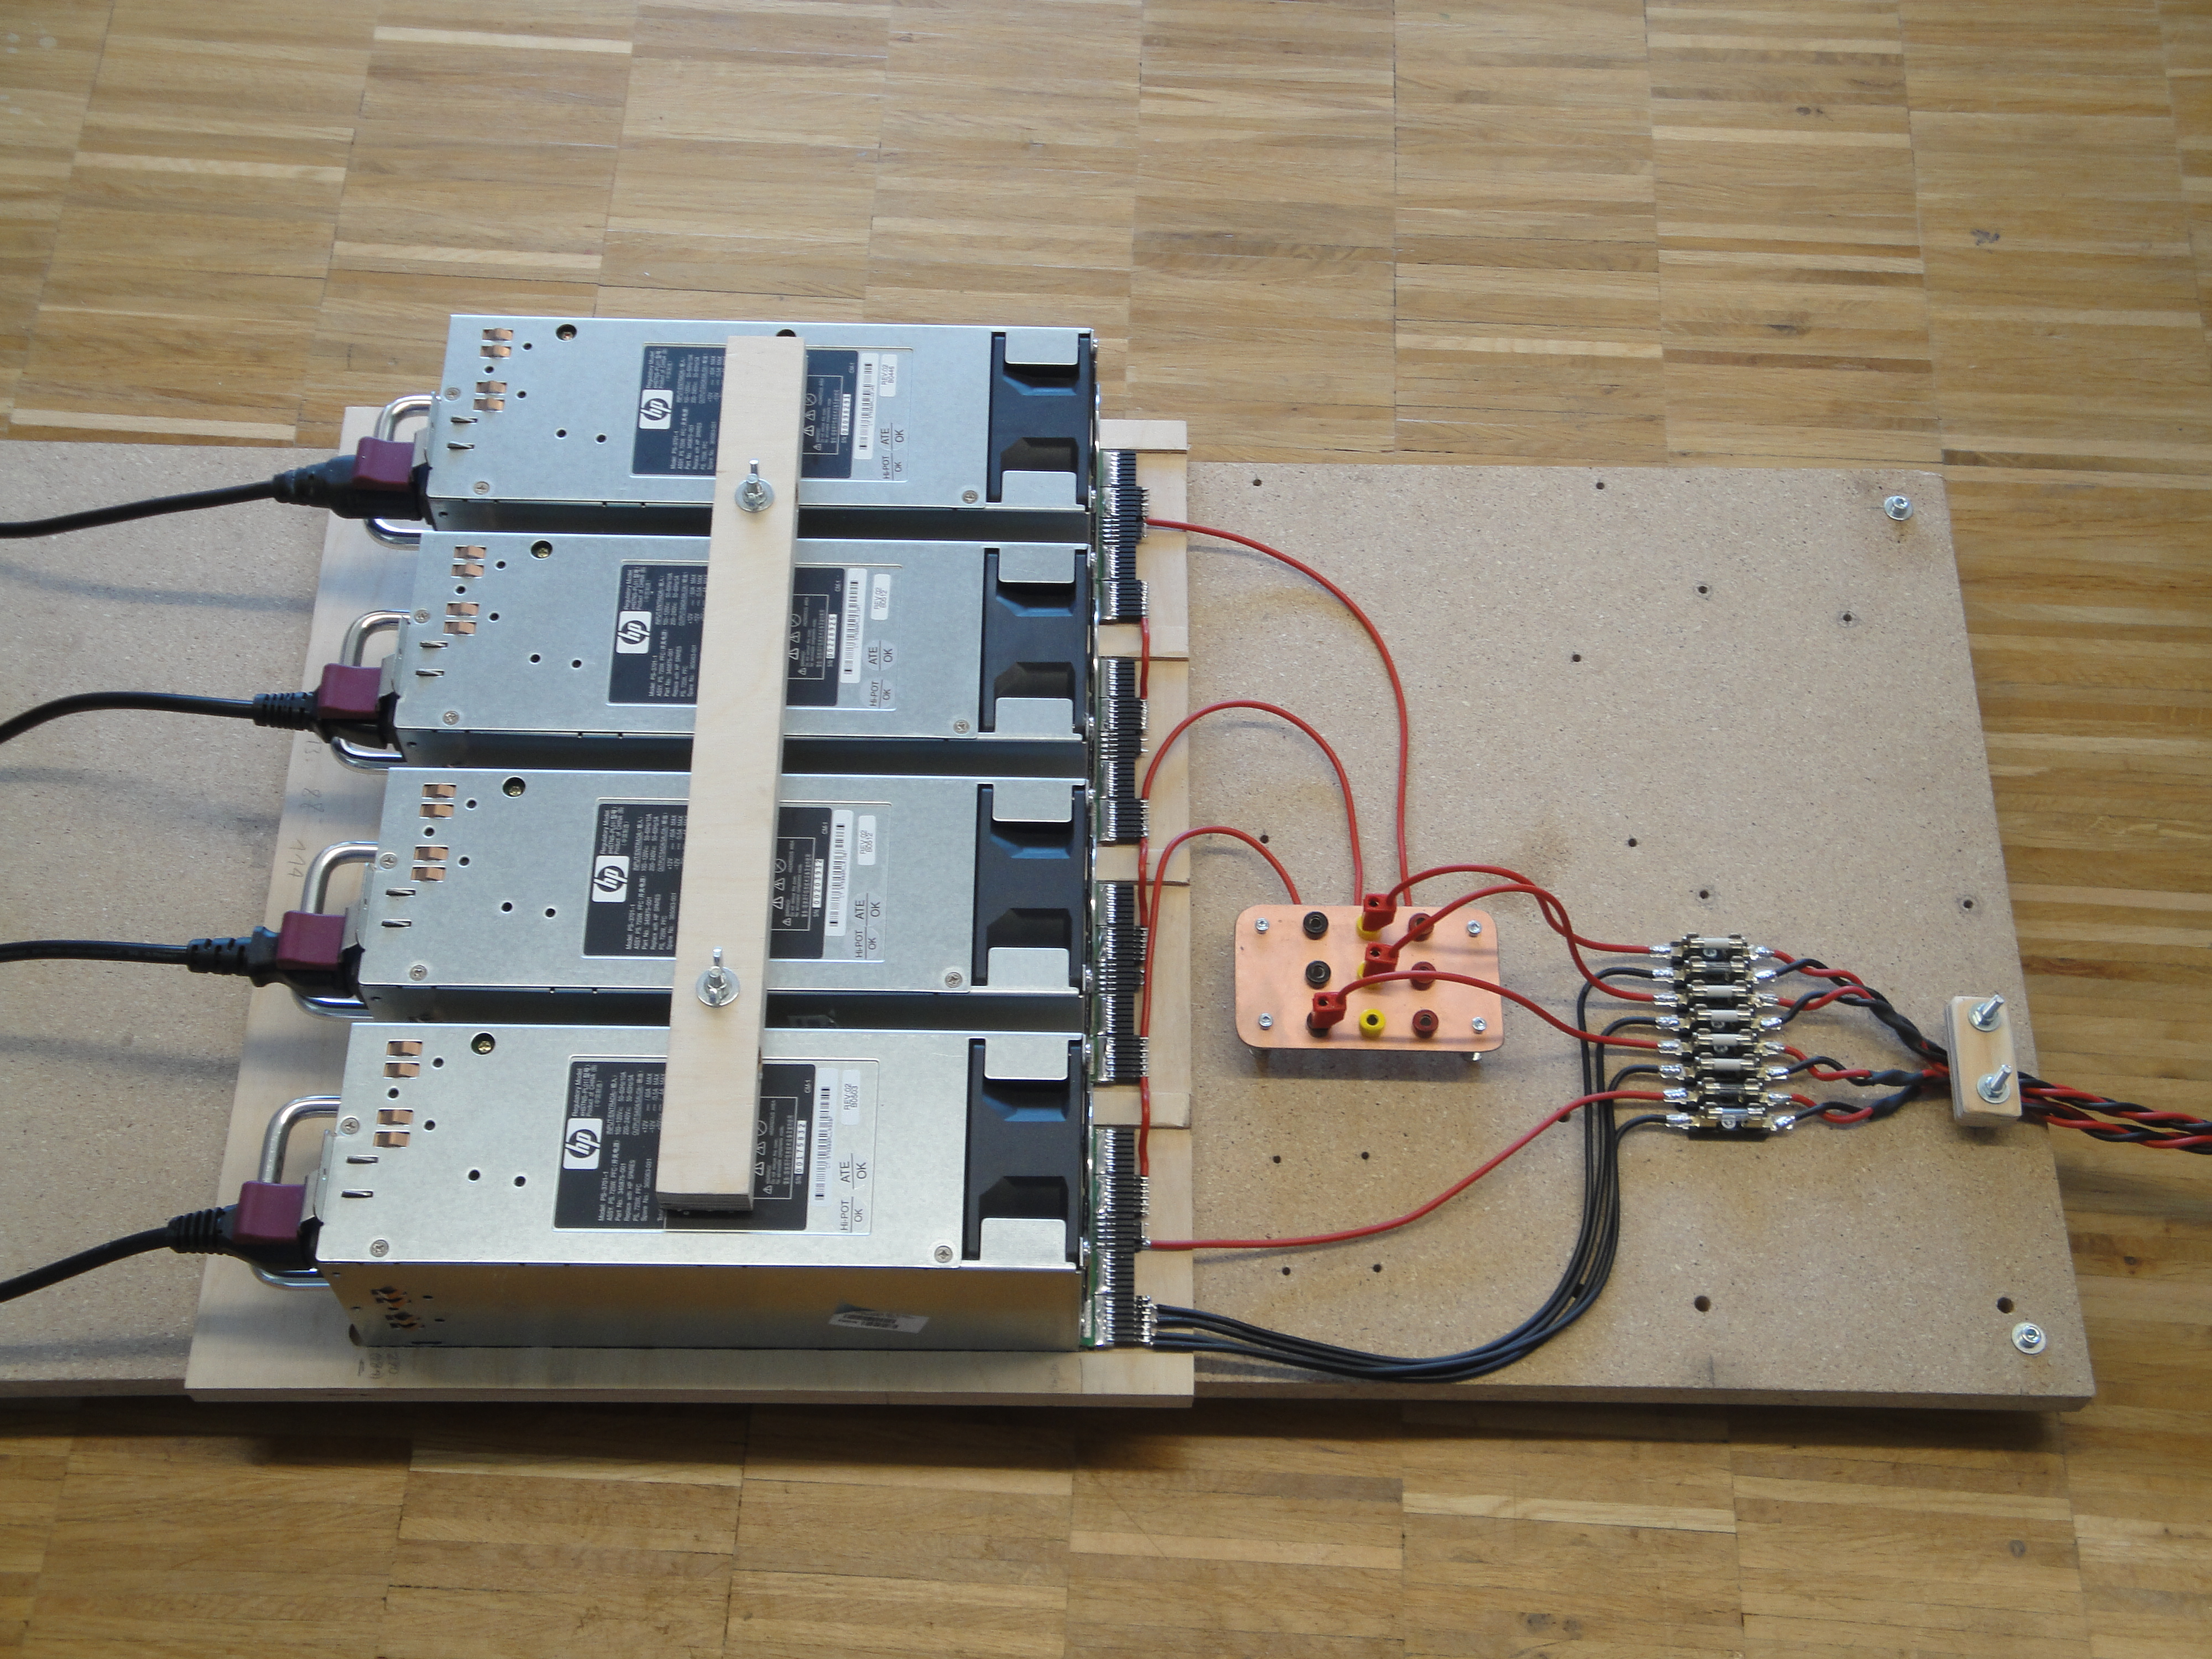
\includegraphics[width=0.8\textwidth]{fig/DSC02936.JPG}
    \caption{Komplette Energieversorgung mit Netzteilen, Steckmatrix und Schmelzsicherungen}
    \label{fig:e_sup_full}
\end{figure}
